\documentclass{article}

\usepackage[francais]{babel}
\usepackage[T1]{fontenc}
\usepackage{moreverb}       % verbatim with tab

\usepackage{wrapfig}
\usepackage{graphicx}
\usepackage{geometry}
\geometry{hmargin=2.5cm}
\usepackage{amsmath}
\usepackage{siunitx}

\usepackage{graphicx}
\usepackage{subcaption}
\usepackage{float}
\usepackage{hyperref}
\usepackage{setspace}
\usepackage{xcolor}
\usepackage{pdfpages}
\usepackage{enumitem}
\usepackage{lscape}

\usepackage{fancyhdr}       % en-têtes
\usepackage{lastpage}       % numéro de dernière page

\title{Temps réel}
\date{2021}
\author{Laura Bin}

\pagestyle{fancy}
\renewcommand\headrulewidth{1pt}
\fancyhead[L]{Laura Binacchi}
\fancyhead[C]{Temps réel}
\fancyhead[R]{\today}

\begin{document}
    \pagenumbering{arabic}

    \begin{center}
        \textbf{\LARGE Exercice 1 -- Les coureurs}
    \end{center}

    \paragraph{}
    Implémenter en C un système dans lequel plusieurs threads doivent attendre un même instant avant de poursuivre leur travail. Cet instant peut se représenter par une barrière implémentée à l'aide de sémaphores. La figure ci-dessous illustre le cas pour 3 threads et 2 barrières.

    \begin{figure}[H]
        \centering
        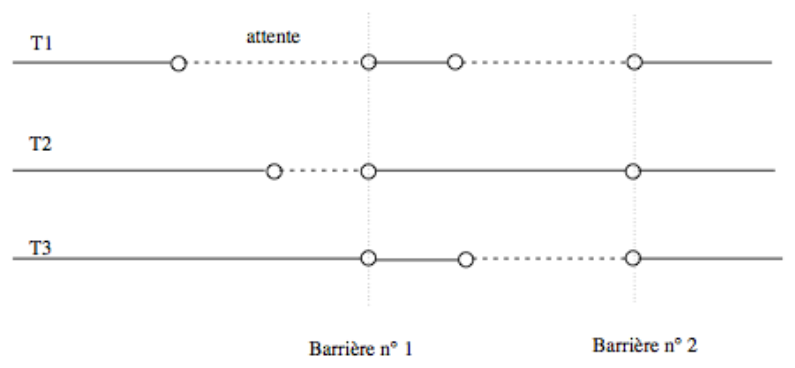
\includegraphics[width=.8\textwidth]{./screenshots/enonce.png}
    \end{figure}

    \newpage
    \section{Compilation}
    Pour compiler ce projet, j'ai utilisé \texttt{cmake}. Le fichier \emph{CMakeLists.txt} permet de générer le \emph{Makefile} avec les options suivantes:
    \begin{verbatimtab}
    [1]     cmake_minimum_required(VERSION 3.10)

    [2]     project(Exercice1_Coureurs VERSION 1.0)

    [3]     set(CMAKE_C_FLAGS "${CMAKE_C_FLAGS} -Wall -Wpedantic -Wextra")

    [4]     include_directories(PUBLIC include)

    [5]     set(SOURCE_FILES
                src/main.c
                src/barrier.c)

    [6]     find_package(Threads REQUIRED)

    [7]     add_executable(race ${SOURCE_FILES})

    [8]     target_link_libraries(race PRIVATE Threads::Threads)
    \end{verbatimtab}

    \begin{description}
        \item[\texttt{[1]}] version de \texttt{cmake} utilisée
        \item[\texttt{[2]}] nom et version du projet
        \item[\texttt{[3]}] ajout des flags habituels pour l'affichage de tous les warnings
        \item[\texttt{[4]}] le répertoire \emph{include} contient les headers nécessaires à la compilation
        \item[\texttt{[5]}] définition de la variable \texttt{SOURCE\_FILES} contenant les fichiers sources du projet
        \item[\texttt{[6]}] ajout du package pour l'utilisation des threads
        \item[\texttt{[7]}] la compilation des fichiers sources produit l'exécutable \texttt{race} 
        \item[\texttt{[8]}] le projet utilise la librairie \texttt{Threads} du package \texttt{Threads}
    \end{description}

    \newpage
    \paragraph{}
    Le fichier \emph{CMakeLists.txt} se trouve à la racine de mon projet. Je lance la commande \texttt{cmake ..} dans le sous-répertoire \emph{build} pour que les fichiers générés y soient placés :
    \begin{figure}[H]
        \centering
        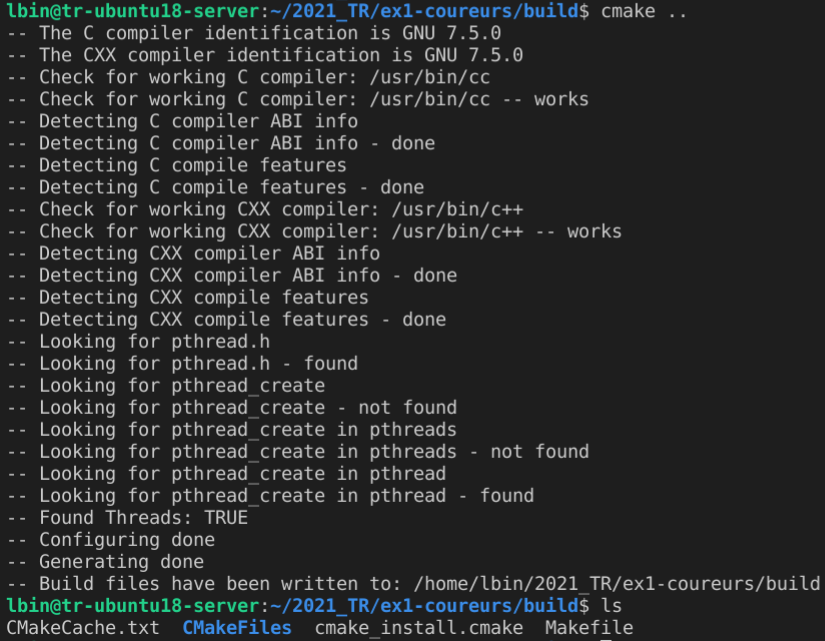
\includegraphics[width=.7\textwidth]{./screenshots/cmake.png}
    \end{figure}

    \paragraph{}
    Par défaut, le \emph{Makefile} est généré en mode debug. Pour le générer en mode release, j'utilise la commande \texttt{cmake -DCMAKE\_BUILD\_TYPE=Release \emph{path}}, où \texttt{\emph{path}} est l'endroit où se trouve le fichier \emph{CMakeLists.txt}.
    
    \paragraph{}
    Je peux maintenant lancer la compilation à partir du \emph{Makefile} avec la commande \texttt{make} qui crée l'exécutable \emph{race} dans le répertoire courant :
    \begin{figure}[H]
        \centering
        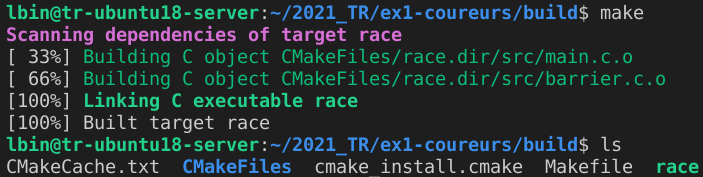
\includegraphics[width=.6\textwidth]{./screenshots/make.png}
    \end{figure}


    \newpage
    \section{Tests}
    \paragraph{}
    Le programme attend en paramètres le nombre de coureurs participant à la course et le nombre d'étapes la composant :
    \begin{figure}[H]
        \centering
        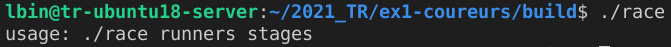
\includegraphics[width=.58\textwidth]{./screenshots/params.png}
    \end{figure}
    
    \paragraph{}
    Les coureurs partent dans l'ordre mais arrivent aux étapes et à l'arrivée dans un ordre aléatoire :
    \begin{figure}[H]
        \centering
        \begin{subfigure}[b]{.48\textwidth}
            \centering
            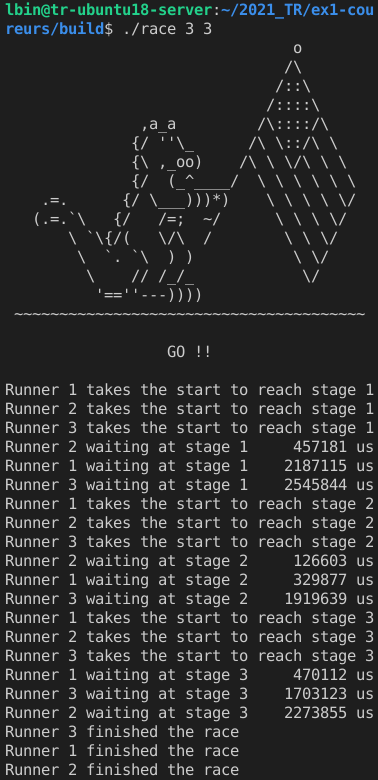
\includegraphics[width=.9\textwidth]{./screenshots/race331.png}
        \end{subfigure}
        \begin{subfigure}[b]{.48\textwidth}
            \centering
            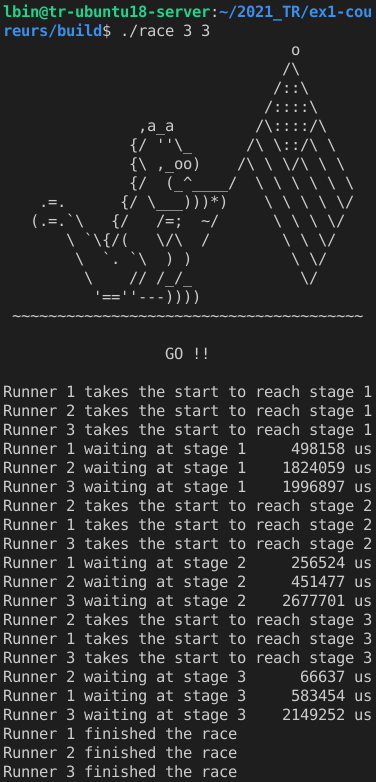
\includegraphics[width=.9\textwidth]{./screenshots/race332.png}
        \end{subfigure}
    \end{figure}

\end{document}
\paragraph{}
